\RequirePackage{fix-cm}
\documentclass{Latex/svjour3}
\usepackage{mathptmx}      % use Times fonts if available on your TeX system
\usepackage{latexsym}
\journalname{Sloan Analytics Conference}
\usepackage{setspace}
\usepackage{url}
\usepackage{multirow}
\usepackage{graphicx}

% Package for notes
\usepackage[draft]{fixme}

%\linespread{2}

\begin{document}

\title{Hot heads, cool heads, and tacticians: Measuring the mental game in
  tennis}

\titlerunning{Measuring the mental game in tennis}

\authorrunning{S. Kovalchik, M. Ingram}

\author{Stephanie Kovalchik\and Martin Ingram}

\institute{S. Kovalchik \at 
              Tennis Australia, Melbourne Park, Australia \\
              \email{s.a.kovalchik@gmail.com}      \\
           \and
           M. Ingram \at
             Stratagem Technologies, London, United Kingdom \\
             \email{martin@stratagem.co}      
}

\date{}

\maketitle

\begin{abstract}

It is often said that winning in tennis is determined as much by a player's
mental game as his or her physical ability yet quantifiable metrics for the
mental side of the game are lacking. We present an approach to identify
mentalities in tennis with dynamic response patterns that quantify how players'
probabilities of winning a point vary in response to the changing situations of
a match. Using nearly 3 million points played by professional male and female
tennis players between 2011 and 2015, we found that top players were generally
affected by the state of the score and a variety of pressure situations,
exhibiting hot hand effects when up in the match, defeatist effects when down,
and performing less effectively in clutch situations than on less important
points. However, player-to-player variation in these dynamic effects revealed
that not all players shared the average mentality profile. The distinct ways in
which players deviated from the field highlighted a variety of differences in
how players respond to pressure and point history and suggested a diversity of
player mentalities at the elite level. Accounting for these dynamic changes in
performance was shown to improve the prediction of match outcomes for the men's
and women's games, substantiating the importance of mentality for performance in
tennis.


\keywords{Tennis\and Player evaluation\and Mixed modeling\and Hierarchical clustering}
\end{abstract}

\section{Introduction}

Mentality is an essential ingredient of all athletic performance. However, the
importance of a player's mental skills in deciding the outcomes of competition
or how fans experience competition varies widely across sports. Tennis, the most
popular individual sport in the
world\footnote{\url{http://www.biggestglobalsports.com}}, is frequently said to
be as much about the mind as the body. Indeed, Jimmy Connors, holder of 109
career titles, has gone so far as to estimate that 95\% of tennis is a mind
game\cite{samulski2007tennis}. Despite these claims, the mental side of tennis
has received limited scientific study and there is currently a lack of
quantitative evidence about the mentalities of today's top tennis players.

Prior work attempting to measure the mental aspect of elite athletic performance
has been limited for all sports, reflecting the challenges of measuring the
mental game. Prior approaches have largely been qualitative in nature, relying
on interviews\cite{young2011understanding} or surveys\cite{taylor1987predicting}
of players and coaches to gain insight about the mental game. These studies have
the drawback that they presuppose that salient mental skills can be measured
with a questionnaire or elicited from a conversation with coaches and
players. Such studies have also not taken advantage of the many years of
historical performance data and what it can reveal about the mental
game. \fxnote{Perhaps we could also say that tennis could be particularly suited
  for measuring mental effects, given that it's an individual sport and we have
  quite fine-grained data?}

In this paper, we present a novel quantitative method to investigate the
mentality of professional tennis players from observed match performance. Our
approach is based on the premise that tennis players reveal aspects of their
mental skills in the way they respond to changes in the state of play over the
course of a match, i.e. the dynamics of a match. Using nearly 3 million points
played in professional singles matches for the men's and women's tours between
2011 and 2015, we quantify player response patterns to point dynamics, identify
common mentalities, and evaluate the importance of mentality for match
performance.


\section{Methods}

\subsection{Data}

Point-level data was obtained for singles matches played on the ATP and WTA
tours during the 2011 to 2015 seasons. For the ATP tour, matches were restricted
to those played at tournaments in the 250 series or above, which includes the 9
Masters 1000 events and 4 Grand Slams (Australian Open, French Open, Wimbledon,
and US Open), where players have the opportunity to earn the most ranking points
and prize money during the season. The WTA data included matches from all
International, Premier, and Grand Slam tournaments. To ensure an adequate sample
size of points for each player, only players with 3 or more match appearances
were eligible for inclusion. Point-level data was obtained from the Tennis
Abstract\footnote{Github source:
  \url{github.com/JeffSackmann/tennis_pointbypoint}} and accessed with functions
from the R package \texttt{deuce}\footnote{Github source:
  \url{github.com/skoval/deuce}} .

The final datasets for the present paper included over 1.6 million points across
10,101 matches played by 434 players for the ATP tour and 1.4 million points for
424 players and 9,668 matches for the WTA tour
(Table~\ref{tab:description}). Approximately 20\% of the points in these
datasets were played at the Grand Slams.


\begin{table}[ht] \centering
\caption{Summary of Point-level Datasets of ATP and WTA
  Singles Matches, 2011-2015}
\begin{tabular}{l cc}
  \hline
Variable  [Shorthand] & ATP & WTA \\ 
  \hline
Points & 1,610,439 & 1,373,095 \\ 
  Players& 434 & 424 \\ 
  Matches & 10,101 & 9,668 \\ 
  Grand Slam Matches & 1,869 & 2,066 \\
\textbf{Candidate Predictors} & &  \\
  ~~Tiebreak, \% & 3.4 & 1.9 \\ 
  ~~Break point, \%& 8.4 & 11.7 \\ 
 ~~Point away from break point, \% [Break point -1] & 17.6 & 21.3 \\ 
  ~~Set or more up, \% [Set+] & 22.4 & 20.8 \\ 
  ~~Set or more down, \% [Set-] & 23.8 & 21.5 \\ 
  ~~Player won last point, \% [Just won] & 53.8 & 51.4\\ 
 ~~Serve game after missed break, \%  [Missed break, serve] & 10.1 & 10.0 \\ 
  ~~Return game after missed break,\%  [Missed break, return] & 9.1 & 8.9 \\ 
  ~~Importance, Mean (SD) & 0.05 (0.05) & 0.06 (0.05) \\ 
  ~~Last game's points, Mean (SD) & 5.5 (2.9) & 5.8 (3.2)\\ 
  ~~Point spread, Mean (SD) & -0.38 (4.5) & -0.19 (4.9) \\  \hline 
\end{tabular}
\label{tab:description}
\end{table}

The analytic datasets were divided into training and validation data for the
purpose of model development and testing. The validation data were the points
played in matches at the 2015 Grand Slam tournaments, the most recent majors at
the time of writing. The training data for each Grand Slam were all points
played up to but not including the Grand Slam event. Thus, four different
training and testing datasets were constructed for each tour and all tournaments
included in the training were independent of the validation tournaments. The
validation data included 105,717 points for the ATP and 71,341 for the WTA.


\subsection{Player Dynamic Model}

We introduce a player dynamic model (PDM) to quantify how an individual player's
performance is uniquely affected by the conditions of a point in a match. The
player-specific dynamics estimated from the PDM will be the basis for
characterizing player mentality. The dependent variable of the model was the
win-loss outcome for a point, with respect to the server of that point. Let
$y_{ijk}$ be the point outcome (Win = 1, Loss = 0) for the $i$th player serving
against the $j$th opponent, on the $k$th service point.

The PDM describes the relationship between the conditions of the point and the
point outcome with the following linear mixed probability model,

\begin{equation}
E\lbrack y_{ijk} \rbrack = (\alpha_{i} + \beta_{j} + \theta)' \mathbf{X}_{ijk}.
\label{eq:pdm}
\end{equation}

\noindent The vector $\mathbf{X}_{ijk}$ contains an intercept, which defines the
baseline serve and return ability of the player and opponent, and $p$ dynamic
features that affect performance on the point outcome (e.g. being a set down,
facing a break point, etc.). The parameters $\theta$ are fixed dynamic effects
that represent how players are affected by conditions \fxnote{I know you
  mentioned you were looking for a different word. ``match situations'', maybe?}
on average. The parameters $\alpha_i$ and $\beta_j$ are player random effects
for each feature for the $i$th player who is serving and $j$th player who is
returning and each are drawn from from a multivariate normal distribution with
zero mean and general variance structure. The player random effects allow that
some players could be more or less affected by the state of a point and that
these effects could additionally depend on whether a player is serving or
returning. The combination of the server and returner effects determine the
expected win probability for the point.

\textit{Remarks.} The PDM can be viewed as an extension of two established
models for predicting point outcomes in tennis. When the feature matrix
$\mathbf{X}$ includes only an intercept, the PDM becomes a regression model for
the opponent adjustment proposed by Barnett and Clarke
\fxnote{\cite{barnett2005combining}}. Klaassen and Magnus also proposed a
dynamic model to test for deviations from the IID model
\fxnote{\cite{klaassen2001points}}, which says that points in a match are
independent and identically distributed. In contrast to the PDM, the model of
Klaassen and Magnus considers a limited number of dynamic effects and does not
incorporate player-specific effects, which are the parameters of primary
interest in the present work.

\subsection{Predictors}

We fit the PDM with eleven candidate predictors that are listed in
Table~\ref{tab:description}. The candidates included a range of dynamic point,
game, and set conditions \fxnote{...and represent our attempt to identify as
  many types of pressuring situations as possible...? Maybe compare against what
  Klaassen \& Magnus chose and how and why we chose different ones?}. The
majority of the point conditions focus on various types of pressure situations,
including indicators of whether a point occurs during a tiebreak, is a break
point opportunity for the returner, or a point away from a break point
opportunity (Break point -1). These predictors can be considered types of
important points because they have a greater influence on the game or set
outcomes than other points. We also include a probabilistic measure of point
importance, defined by Morris\cite{morris1977most}, that is equal to the average
change in match win probability when the current point is won compared to win it
is lost, given the state of the match at this point. One final point condition
is an indicator of whether the server won the previous point (Last won
\fxnote{This is now ``Just won'' I think?}), which captures short-term
correlation between points that could arise from a one-point hot hand effect,
for example.

Three predictors contained information about game history. Two concerned missed
opportunities to break service and how this affected the subsequent service game
(Missed break, serve) and return game (Missed break, return). In the coding for
these predictors, it is assumed that the psychological impact of a missed break
is a within-set effect and does not carry over into the games of other sets or
tiebreaks.  We also examined how the number of points played in the previous
game might influence play in the current game. A more closely contested game
will have more points played, and could serve as an indirect measure of player
fatigue.

There were also three set conditions included in the set of predictors. Two of
the predictors indicated when the player serving was either up a set or more
(Set+) or down a set or more (Set-) in the match. Finally, in order to capture
longer term momentum effects than those due to the outcome of the previous
point, we tracked the point spread across games within a set, subtracting the
points won in the set by the player serving from those of the player returning.

\fxnote{Like the note above mentioned, I think this part is good but could do
  with a bit more explanation of why we chose the predictors we did...?}


\subsection{Model Estimation}

The PDM was implemented with the R package \texttt{lme4} using a Gaussian family
for the outcome distribution. The Gaussian model has a number of desirable
features. Most importantly, the dynamic effects have a simple and meaningful
interpretation, as they represent the absolute change in point win probability
for a one unit increase in a feature. The model is also the most computationally
efficient within the generalized linear family. However, the model is most
appropriate for continuous outcomes, whose mean, unlike a binary outcome, does
not have a constrained support.

Klaassen and Magnus have previously shown \fxnote{\cite{klaassen2001points}}
that the linear model works well in practice for modeling point win
probabilities. We also conducted our own investigation by obtaining marginal
predictions for the dynamic effects using a logistic model and comparing these
to their corresponding effects with the linear probability model. The effects
differed by no more than one significant digit, indicating that the lack of
constrained estimation had a negligible impact on the PDM estimates.

In addition to the PDM, we fit two additional models for the purpose of
evaluating the overall improvement in prediction performance with the inclusion
of player-specific dynamics. One of these was a simpler version of the dynamic
model that had average effects for the eleven dynamics and only an intercept
term for the player effects. We will refer to this model as the average dynamic
model (ADM). The second model had only an intercept term for the average and
player effect. Without any dynamic effects, this model is equivalent to an IID
model.

\subsection{Model Performance}

To summarize the overall magnitude and significance of the dynamic effects, we
fit the ADM with all of the available data and computed 95\% confidence
intervals for each effect. The added value of including player-specific effects
for each dynamic feature was measured by the change in the Akaike Information
Criterion (AIC). The AIC is a measure of overall model fit that allows
comparisons between non-nested models and rewards more parsimonious models. For
each dynamic predictor, we estimated the change in AIC with the inclusion of
player-specific effects versus a constant effect for all players.

To assess the implications of mentality on points for predicting the outcomes of
matches, we used a Monte Carlo simulation to test the predictive performance of
the PDM. The simulator ran $5,000$ trial matches for each pairing of the 2015
Grand Slams (a best-of-five format for the ATP and best-of-three for the
WTA). Each simulated point on serve in a match adjusted the server's probability
of winning the point according to the state of that point as described by the
PDM, and the fraction of trial matches won gave an estimate of the probability
that a player won the match. The player dynamic match predictions were compared
to two alternative models: the ADM that assumes constant dynamic effects for all
players and an IID model that assumes no dynamic effects, i.e. a constant point
win probability for each server. Our primary metric of performance was log loss,
as it places a high penalty on overconfident predictions\cite{yuan2015mixture}.


\subsection{Identifying Mentality Types}

The ways in which a player's performance is affected by the conditions of a
match provide insight into the player's mentality. The set of player-specific
dynamic effects from the PDM\textemdash which represent how much more or less a
player's performance on a point shifts in response to conditions compared to the
field\textemdash provide a mentality profile. To identify common mentalities on
the tour, we applied a hierarchical clustering method to the dynamic profiles of
the players who competed in the 2015 Grand Slams. Only the most salient features
for distinguishing player types were included, which were defined as the
features that showed an AIC improvement over the ADM that indicated significant
variation in the effect from one player to the next.

Prior to clustering, the dynamics effects of the mentality profiles were
converted from their probability scale to a z-score so that each effect would
have the same mean and variance and allow for direct comparison between
effects. A distance measure was then applied to all possible pairs of the
standardized profiles (e.g. Player A's standardized dynamics on tiebreaks, break
points, etc. versus Player B), which results in a dissimilarity matrix. We then
apply a linkage approach to identify clusters among players.

There are a number of options available for both the distance metric and linkage
approaches and the choice of method in each case could potentially influence the
resulting clusters. Three common measures of distance are the Euclidean
($L_2$-norm), the Manhattan ($L_1$-norm), and absolute maximum (or Chebyshev's
distance). The methods primarily differ in their response to outliers with the
maximum distance being most sensitive to extremes and the correlation least
sensitive.

The linkage method is the technique applied to the pair-wise distances to
determine a measure of the cluster distance. \textit{Single linkage} is a
nearest neighbor method that assigns clusters based on the minimum
distance. Average linkage chooses the cluster that minimizes the average
distance between. Complete linkage is the opposite extreme of single linkage in
that it assigns clusters by maximizing the difference between clusters. Each of
the hierarchical techniques begin with all units assigned to a single cluster,
i.e. a `bottom up' approach.

There is no universally best method among these; the performance, instead,
depends on the properties of the data used \cite{kumar2014performance}. For this
reason, each combination of distance measure and linkage measure were
examined. The approach selected was one that showed the largest number of
patterns containing two or more players per cluster.

The choice of the number of clusters was selected by beginning with a large
number ($K = 12$) and visually inspecting the patterns of each cluster with
parallel coordinate plots. When two or more clusters could not be easily
distinguished the number of clusters was reduced by one. This process was
repeated until all patterns could be uniquely described.


\subsection{Player Unpredictability}

It is possible that some players will not easily fit into any of the identified
mentality types. One way this could arise is if a player's shifts in performance
are essentially random, ups and downs that are unrelated to the specific
conditions of the point. To examine which player's exhibited more or less of
this kind of volatility in their mentality, we computed the mean Brier score of
the PDM predictions for each player on serve and return when applied to the
Grand Slam validation data. Outliers were flagged as players with variances that
were 2 or more standard deviations from the mean.

\section{Results}

\subsection{Characteristics of Dynamic Predictors}

Among the eight categorical dynamics, a server's win on the previous point was
the most common, occurring slightly more than half of the time for each tour
(Table~\ref{tab:description}). For one of every five points on serve, at least
one competitor would be expected to be a set up or down in a match based on
recent years of matchplay. A similar percentage of points would be one point
from a break point opportunity. Break points and points played in games
following a missed break opportunity were some of the least common events among
the predictors, happening approximately 10\% of the time during a match. The
rarest dynamic event was a tiebreak, which occurred for 3\% of points on the
men's tour and 2\% of points on the women's tour.

The average importance of a point in a tennis match was 5 probability points,
corresponding to an expected increase in match win probability of 5 percentage
points when the point was won versus lost (Table~\ref{tab:description}). In
recent years, we also found that the average number of points played in a game
was 6 for both tours. \fxnote{Was it different before, or why in recent years?}
The average point spread over the games in a set was approximately zero but it
was not unusual to observe differences as large as 10 points. \fxnote{Maybe
  explain a little -- when a player falls far behind in a set...?}

\subsection{Average Dynamic Effects}

The average dynamic effects on point outcomes identified factors that
significantly increased the advantage of the server as well as effects that
increased the advantage of the returner. For both tours, a server's win
opportunity was negatively affected when playing a set down, when facing a break
point, or when facing more important points overall
(Table~\ref{tab:estimates}). By contrast, when a server was ahead a set (or
more) in a match, had won the previous point, or otherwise had a lead in the
point spread, we found the server generally had a significantly greater
probability of winning a point. Because the point spread can take negative
values when the server is behind in the set, the impact of spread would, in this
case, have a comparable negative effect on the server's win probability. In data
not shown, we assessed the linear assumption for point spread and found that the
relationship was best described by a line with approximately equal slope for
positive and negative spreads with respect to the player serving.

\begin{table}[ht] \centering
\caption{Average Effects of Dynamic Conditions on Point Performance
  Played for the 2011 to 2015 ATP and WTA Tours}
\begin{tabular}{l ccc ccc} \hline
\multirow{2}{*}{Dynamic} & \multicolumn{3}{c}{ATP} & \multicolumn{3}{c}{WTA} \\
 & Estimate & 95\% CI & $\Delta$AIC$^a$ & Estimate & 95\% CI &$\Delta$AIC\\ \hline
Base rate & 63.20 & (62.72, 63.69) &--& 55.79 & (55.31, 56.27)  &\\ \noalign{\smallskip}
Tiebreak& -0.06 & (-0.53, 0.41) &2.8& -0.61 & (-1.27, 0.05) &-2.3\\ 
Break point & -0.76 & (-1.08, -0.44) &0.9& -0.63 & (-0.95, -0.31) &0.2\\
Break point -1 & -0.39 & (-0.61, -0.18) &8.9& -0.02 & (-0.24,
0.21) &0.6\\ 
Set+ & 1.43 & (1.24, 1.63) &5.2& 1.71 & (1.49, 1.92)  &-0.4\\ 
Set- & -1.94 & (-2.13, -1.75) &19.2& -2.01 & (-2.22, -1.80)  &0.4\\
Importance & -4.34 & (-6.43, -2.26) &32.2& -5.56 & (-7.77, -3.36)  &0.6\\ 
Point spread  &  0.30 & (0.28, 0.32) &13.3& 0.31 & (0.29, 0.33) &-2.5\\
Just won &0.63 & (0.47, 0.78) &44.4& 0.51 & (0.33, 0.69) &0.6\\ 
Missed break, serve  &0.21 & (-0.09, 0.51) &-4.1& 0.20 &(-0.12, 0.52)&-2.6\\ 
Missed break, return   & -0.22 & (-0.49, 0.04) &-3.4& 0.12 & (-0.18, 0.41)  &-3.3\\ 
Last game's points & -0.01 & (-0.04, 0.02) &-5.3& -0.02 &
(-0.05, 0.01) &  0.4 \\ \hline
\multicolumn{7}{l}{CI = Confidence interval, AIC = Akaike Information
Criterion} \\
\multicolumn{7}{p{5in}}{a Change in AIC with inclusion of player-specific
  dynamic effects compared to a constant dynamic effect. Larger values
  indicate the player-specific model provided  a better fit to
  observed point outcomes.} \\
\end{tabular}
\label{tab:estimates}
\end{table}

While the majority of the effects were nearly identical for both the men's and
women's tours, there were a few interesting exceptions. Being a point away from
a break point opportunity had a modest negative effect on the server's advantage
among male players but not female players (Table~\ref{tab:estimates}). For the
men's tour, missed break opportunities had a modest boost to the next return
game of the returner who failed to convert but no evidence of an effect for the
women's tour. However, we found some evidence of a decrease in serve advantage
for the women's tour during tiebreak points, which was not observed for the
men's game.

\begin{figure}
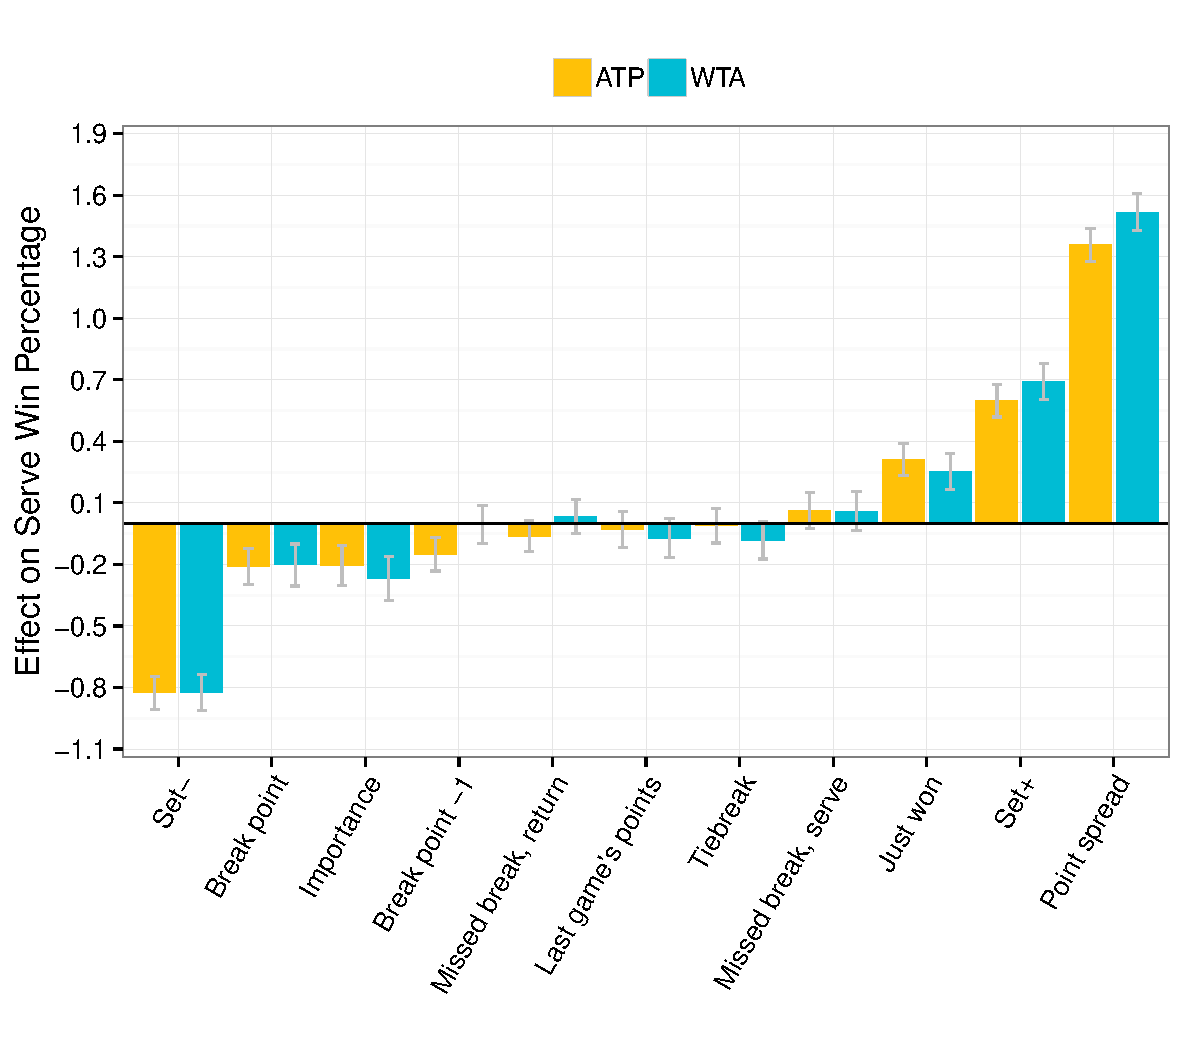
\includegraphics[scale=0.8]{figs/avg_effects.pdf}
\caption{Average dynamic effects on the probability of winning on serve based on
  point-level data for 2011-2015 ATP and WTA singles matches. The y-axis shows
  the estimates change in the probability of winning a point on serve (in
  percentage points) for a one standard deviation change in the dynamic
  predictor. Error bars denote the 95\% confidence interval for the estimated
  effect.}
\label{fig:1}
\end{figure}

The estimates in Table~\ref{tab:estimates} represent the estimated change in
serve probability (in percentage points units) associated with a one-unit
increase in a dynamic factor. Because a one-unit increase might not be
meaningful for all of the predictors (e.g. point importance), we compare the
average effects on a standardized scale where each bar corresponds to the change
in serve win probability for one standard deviation increase in the
corresponding dynamic factor (Figure~\ref{fig:1}). This plot reveals that the
strongest predictor for both tours was point spread, where a server with a one
standard deviation lead in the point score was estimated to have a 1.4-1.5
percentage point increase in point win probability. Being a set up or set down
were runners up with a roughly 1 percentage point effect size, a server being a
set up adding to the server's advantage and server being a set down adding to
the returner's advantage. Other game and point conditions had more moderate
effects, with some indication of a relatively stronger negative effects on
important points and tiebreak points for female players compared to male
players.

\subsection{Player Dynamic Effects}


The estimates shown in Table~\ref{tab:estimates} represent the effect of each
dynamic feature if all players were equally influenced by the state of the
match. However, because not all players have the same mentality on court, we
would expect some players to respond differently to point conditions than
others. The player dynamic model allows for player-to-player differences in
their response to the state of the match by estimating a separate dynamic effect
for each player.

To determine when the player-specific dynamics better explained observed
performance, we calculated the improvement in AIC with the PDM. The changes in
AIC shown in Table~\ref{tab:estimates} reveal the presence of important
player-to-player differences in the dynamic effect, positive changes reflecting
a better fit with the PDM. For the men's game, all but three of the predictors
demonstrated important player dynamics. The exceptions were both indicators of
missed breaks of service and the total points played in the last game. While
dynamic factors with a significant average effect were generally found to also
have important player-to-player variation, tiebreak points were found to have
important player-to-player variation in performance despite a weak average
effect for the men's tour.

For the WTA, improvements with the PDM were fewer and smaller in magnitude than
for the ATP. Six of the 11 factors\textemdash break points, being one point from
a break point, being down a set, point importance, the outcome of the previous
point, and the total points played in the previous game \textemdash showed
important player-to-player variation (Table~\ref{tab:estimates}). Thus, male
player responses to tiebreak points, being a set up, and having a lead in point
were more variable than for female players, whereas female player responses to
the total points played in a game were more variable.

\subsection{Model Performance}

On the ATP, the importance of mental effects was confirmed by the greater
accuracy and lower log loss for the predictions of the dynamic models compared
to the IID model (Table \ref{tab:performance}). The consistent superior
performance of the PDM over the ADM substantiates the importance of player
differences in response to the changing situations of match play on the men's
tour.

While the dynamic models also improved match predictions for the women's tour,
the differences were smaller than for the men's and the performance of the
average and player-specific dynamic models were statistically equivalent.

\begin{table} \centering
\caption{Summary of Match Prediction Performance for the 2015 Grand Slams}
\begin{tabular}{l ccc ccc} \hline
\multirow{2}{*}{Tournament} & \multicolumn{3}{c}{Accuracy} & \multicolumn{3}{c}{Log Loss} \\ 
&	IID &ADM &PDM &IID &ADM &PDM \\ \hline
\textbf{ATP} & & & & & & \\
~~Australian Open	&73.3&	74.1&	76.7&	0.515&	0.505	&0.493\\
~~French Open	        &70.6&	70.6&	73.9&	0.547&	0.542	&0.536\\
~~US Open	        &74.5&	74.5&	76.4&	0.505&	0.498&	0.494\\
~~Wimbledon	        &74.2&	73.3&	73.3&	0.534&	0.521&	0.514\\
~Overall	        &73.1&	73.1&	75.1&	0.526&	0.517&	0.510\\
\textbf{WTA}  & & & & & & \\
~~Australian Open	&73.2&	74.0&	75.6&	0.596&	0.574&	0.560\\
~~French Open	        &72.7&	70.2&	71.9&	0.567&	0.562&	0.560\\
~~US Open	        &64.2&	63.3&	64.2&	0.662&	0.631&	0.638\\
~~Wimbledon	        &70.4&	70.4&	69.6&	0.570&	0.555&	0.558\\
~Overall	        &70.1&	69.5&	70.3&	0.598	&0.580& 0.579\\ \hline
\multicolumn{7}{p{3.8in}}{IID = Independent identically distributed, ADM =
  Average dynamic model, PDM = Player dynamic model}
\end{tabular}
\label{tab:performance}
\end{table}

\subsection{Mentality Profiles}

\subsubsection{Men's Tour}

The eight dynamic factors that improved the predictive performance of point
outcomes for the men's tour revealed eight unique mentalities among the male
players who had competed in one or more of the 2015 Grand Slams. The players
with each mentality type are displayed in Figure~\ref{fig:atp_dendro} as a
dendrogram in which mentalities that are more similar are closer together in
their order from top to bottom. The underlying feature profiles for each group
are displayed in Figure~\ref{fig:atp_coord}. Here, each line is a specific
player's set of dynamic effects on serve and return and effects are scaled so
that they all have an equal standard deviation of one. A smoothed regression
line is plotted over the observed profiles in each panel to highlight the key
differences from the status quo (`The Field') shown in gray.

\textit{The Field}. We begin with a description of the mentality suggested by
the cluster with the largest number of players and, consequently, the most
common profile among top male players. This group exhibits a drop in performance
when pressure is on the serve, as indicated by the negative effects when a set
down and facing important points, including break points and tiebreaks
(Figure~\ref{fig:atp_coord}). These players also exhibit sensitivity to the
state of the point score, as is indicated by the positive effects on winning the
previous point, having an edge in point spread, or being a set up. These `hot
hand' effects induce a corresponding loser's curse on the return game, in which
players who fall behing are even less likely to win a point than when even or
ahead in the score.

\textit{John Isner}. One of two players with a unique profile was big server
John Isner. The large positive effects on serve indicate greater overall mental
toughness when serving than any other player evaluated. On the defense game,
Isner's mentality showed \fxnote{maybe turn into ``may indicate'' given that it
  could also be something else?} a lack of confidence on break point and other
important points. His performance on the return game was otherwise similar to
the field, with the exception of tiebreaks where he showed strong performance
whether returning or serving.

\textit{Tiebreak Specialists}. Like Isner, these players shine on tiebreak
points, raising their performance when serving or returning. On other point
types, they also exhibit a similar disparity between the service and return
games, with greater overall confidence on serve, but to a less extreme degree
than Isner.

\textit{Fabio Fognini}. The second player found to have a unique mentality was
Fabio Fognini, Italian No. 1 at the time of this writing. Fognini's distinctive
characteristics backup the mercurial label he has often been given by the
media\footnote{Medlock, W. (June 14, 2015) `Ranking the Most Unpredictable
  Tennis Players Today'. Retrieved from:
  \url{http://bleacherreport.com/articles/2495031-ranking-the-most-unpredictable-tennis-players-today/}}. While
being unusually mentally strong on more important points (especially on the
return game) and on making break point opportunities, the large negative effects
when a point or set down on return indicate that he is one of the players most
susceptible to collapse.

\textit{Champions}. The players who currently hold the most Grand Slam titles
Novak Djokovic, Roger Federer, Andy Murray and Rafael Nadal (colloquially
referred to as `The Big Four') were all found in the same mentality cluster,
suggesting a `Champion's mentality'. The players in this group exhibit similar
strength on serve as the big servers among the tiebreak specialists except for
the boost in performance on tiebreaks. On the return game, these players set
themselves apart with the mental toughness they show in clutch situations:
important points and creating break point opportunities. While the majority of
these players also showed a greater ability to convert break points than other
competitors, it is interesting to note that Roger Federer was most similar to
the field on this characteristic.

\textit{Opportunity Makers}. This group of players had many of the tendencies of
the champions group but to a lesser degree. The most consistent positive trait
observed compared to the field was the tendency to raise their game to make an
opportunity to break serve, shown by the positive effect on the point away from
break point on the return game. Several of the most exciting players of today's
game\textemdash Jo-Wilfried Tsonga and Ga\"{e}l Monfils\textemdash are included
in this group. \fxnote{I like that you pick the players out, but maybe ``most
  exciting'' could be a bit subjective? Maybe tone down to ``considered to be
  most exciting'' or something?}

\textit{Tight}. This mentality was the only one that was noteworthy for being
weaker on certain points than the average top player. Specifically, in clutch
situations on serve and when down a point or a set on the return game, these
players showed a greater drop in win probability than any others. Finding former
World No. 1 Lleyton Hewitt in this group was unexpected but could be explained
by the point-level data only covering the final years of his
career. \fxnote{This is really good now!}

\textit{Score Keepers}. In addition to being generally less confident on serve,
the final group of players were unique in their response to the outcome of the
previous point, showing a hot hand response when winning a point on serve and a
corresponding `cool hand' after losing a point on return. Thus, the performance
of these players is unusually sensitive to the short-term state of the score.

\subsubsection{Women's Tour}

Considering the six player-specific dynamics for the women's tour, eight unique
mentalities were also found among players competing in the 2015 Grand Slams
(Figure~\ref{fig:wta_dendro}).

\textit{The Field}. Like male players, the majority of the service game of top
female players is negatively affected under pressure but benefits from a recent
point win\textemdash a mini hot hand effect.

\textit{Fighters}. Several of the top players were found to raise their level of
play after tightly contested games (Figure~\ref{fig:wta_coord}). These players
had large positive effects associated with more points played in the last game
on both return and service games, but especially on the service game. These
players also exhibit greater cool-headedness in clutch situations on the return
game, but their most distinctive characteristic is the fighter's mentality
suggested by their improved performance after long points. It is worth noting
that World No. 1 Serena Williams, known for her mastery of the comeback, had the
largest positive effect for long points on serve. \fxnote{Should this maybe
  ``serving after playing a long return game''?}

\textit{Stoics}. Another group of players showed even greater cool-headedness on
the return game than the `fighters'. The defense performance for these players
was virtual unaffected by the state of the score or the importance of points
other than break points. On the service game, these players were also the least
negatively affected by pressure and the least phased by being a set down. Two
players often praised for their mental toughness\textemdash Maria Sharapova and
Victoria Azarenka\textemdash were found in this group.

\textit{Faders}. In sharp contrast to the `fighters' described above, another
set of players had a notable negative effect in their service game after a
closely contested game, which could be the effect of mental or physical fatigue.

\textit{Tight}. While nearly all players show some decline in serve performance
in pressure situations, only one group of players had strong and nearly equal
negative effects when facing a break point, a break point opportunity, or other
important points.  Although less pronounced on the return game, the greater
negative effect on points away from break point suggest that vulnerability in
clutch situations affects both parts of these players' game.

\textit{Clutch Servers}. We also observed a group of players that were generally
unaffected by pressure on serve, having little or no effect on break points and
other important points. There was also some evidence of improved performance on
serve after long points like that observed for the `fighters' group. Several
players found in this group, like Sam Stosur and Petra Kvitova, are known for
inconsistent displays of excellent play.

\textit{Savers}. Two players, Barbora Strycova and Caroline Garcia, stood out
from the rest of their cohort for being unusually unmoved on serve when facing a
break point.

\textit{Preemptors}. One of the larger group of players were noteworthy for
their mentality on serve when a point from facing a break point. Unlike the
field, these players tended to increase their win probability to avoid a
possible break of service. Several rising stars of the WTA tour, including
Garbine Muguruza and Belinda Bencic, were members of this group.


\subsection{Unpredictable Performance}

When we measured the prediction error of the PDM for each player (a metric of a
player's unpredictability), we found more outliers who were unusually
predictable than outliers who were unusually unpredictable. For both tours, a
small but roughly equal number of players were highly predictable on serve and
return.

Figure~\ref{fig:volatility} highlights the ten players on each tour who were the
most extremely predictable. On the men's side, the group clustered in the lower
left quadrant are players who had very little variation on the serve or return
game after accounting for the dynamic effects of the PDM. Notably, 3 of the
strongest servers on tour (John Isner, Milos Raonic, and Ivo Karlovic) were
among this group. The lower right quadrant consisted of players who were
predictable on serve but much less so on return. It was surprising to observe
three of the greatest players of the current era (Roger Federer, Novak Djokovic,
and Rafael Nadal) in this group. \fxnote{Just wondering -- is Murray there
  anywhere? I think one can make the case that he's a step below these guys, but
  he should maybe be almost up there...?}

While a similar pattern in predictability was found for the women's tour, fewer
of the outlying players were as highly ranked as for the men. The exception was
for the lower right quadrant where we, as with the men, we found several of the
tour's greatest champions: Serena Williams and Maria Sharapova. The similarity
of this result for the men's and women's tours makes the intriguing suggestion
that mental steadiness on serve combined with variety on return could be one of
the defining characteristics of a champion at the professional level.

\fxnote{I do think this section is very cool, but do we completely understand
  what's going on...? Also, should we maybe mention that perhaps the outliers
  are predictable, except we are not capturing it with our (granted, pretty
  extensive) model...? And offer some potential explanations -- different
  ``gears'', tactics...?}


\section{Discussion}

In this paper, we presented a novel approach to quantify changes in tennis
performance in response to dynamic situations on serve and return in a
match. When applied to millions of points of recent performance data, we found
that top players were generally affected by the state of the score and a variety
of pressure situations, exhibiting hot hand effects when up in the match,
defeatist effects when down, and performing less effectively in clutch
situations than on less important points. However, player-to-player variation in
these dynamic effects revealed that not all players shared the average mentality
profile. The distinct ways in which players deviated from the field highlighted
a variety of differences in how players respond to pressure and point history
and suggested a diversity of player mentalities at the elite level. Accounting
for these dynamic changes in performance were shown to improve the prediction of
match outcomes for the men's and women's games, substantiating the importance of
mindset for performance in tennis.


A fundamental feature of our approach for measuring mentality is the isolation
of a player's response to changing match situations from his or her overall win
ability. This is done by focusing on how a player's performance varies around
his or her own baseline probability of winning a point. As a consequence of this
separation of baseline ability from point-to-point variation in performance, the
approach allows that players with different physical skills could still share a
common mentality.

In spite of this flexibility in the approach, our findings revealed instances
where the physical and mental sides of the game were closely linked. This was
most striking on the men's tour in the clustering of players known for their big
service game (John Isner, Milos Raonic, etc.) and the similarity in the profiles
of the most dominant players of the tour. The finding that all of the `Big 4'
(Novak Djokovic, Roger Federer, Andy Murray, and Rafael Nadal) deviated in very
similar ways in response to changes in pressure and point history suggests the
existence of a champion's mentality that is notable for clutch performance on
the return and relative imperviousness to the conditions of the point on serve.

Another interesting relationship between player skill level and point-to-point
performance among ATP players was the finding that 3 of the most accomplished
players on the men's game (Roger Federer, Novak Djokovic, and Rafael Nadal) were
also some of the most predictable players on serve and most unpredictable on
return. Considering this result with the qualities of the champion profile that
was characterized by stoic serve ability and an attacking defensive game, we
conclude that the most successful players on the men's tour distinguish
themselves for their mental toughness [cite] on serve and their variety on the
return game, which challenges the conclusions of prior work stating that players
should `play every point as it comes'\cite{klaassen2001points}.

The average dynamic effects for the men's and women's tour were remarkably
similar, with the only statistical difference being the women's absence of an
average effect on points a point away from a break point that was found to
negatively effect men's serve performance overall. However, player variation in
effects was less extensive on the women's tour compared to the men's tour. Fewer
of the dynamic variables showed significant player-to-player variation for
female players, and the variation that was observed was largely restricted to
the service game. This suggests that the variety of mentalities on the women's
tour might be less numerous than the men's or that other dynamic factors not
considered in this paper are needed to explain variation in female point
performance.

When we examined the unexplained variation among female players, we found that
two of the current greatest female players, Serena Williams and Maria Sharapova,
had similar characteristics as the male champions. These players were some of
the steadiest players on serve but the most variable on return. The observation
of this pattern on both tours adds strength to the conclusion that champions
share common mental skills on court and further suggests that the champion's
profile might be independent of gender.

In interpreting the observed point-to-point changes in performance, we have
regarded these deviations as indicators of shifts in psychological traits of a
player like confidence, mental toughness, or resilience. It is important to
acknowledge other possible explanations for systematic fluctuations in
performance. Shifts of performance with specific match situations could be a
conscious tactic, like a defender who might plan to take bigger risks when a
point from a break point opportunity. Also, because point-level data is the
result of the behavior of two players, it is possible that observed changes
associated with a particular player are owing to the ways other players adapt to
that player's game, like players becoming tight on big points when facing a top
10 player.

Even with uncertainty as to the definitive causes of point-to-point differences
in player performance, the measurement of these deviations could be a valuable
aid to coaches by visually highlighting the relative strengths and weaknesses in
how their player's performance changes with specific match conditions. When a
player's profile is placed in the larger context of the field, it can also
suggest players with similar and different responses to match situations, which
could suggest strategies for modifying a player's game where room for
improvement is needed. Such visual displays as presented her could also be an
engaging way to contrast player performance to fans.

Present efforts are underway to amass shot-by-shot data that would enable the
study of performance to go beyond the simple outcome of the point when
characterizing player performance. Ball and player position tracking from camera
and wearable technologies will also become increasingly common over time. As
richer and more detailed data on tennis performance becomes available in the
future, the framework we have presented in this paper provides analysts with a
valuable tool for evaluating player mentality at an increasingly precise level
of detail.

\bibliographystyle{Latex/spmpsci} 
\bibliography{bib}

\clearpage

\begin{figure}
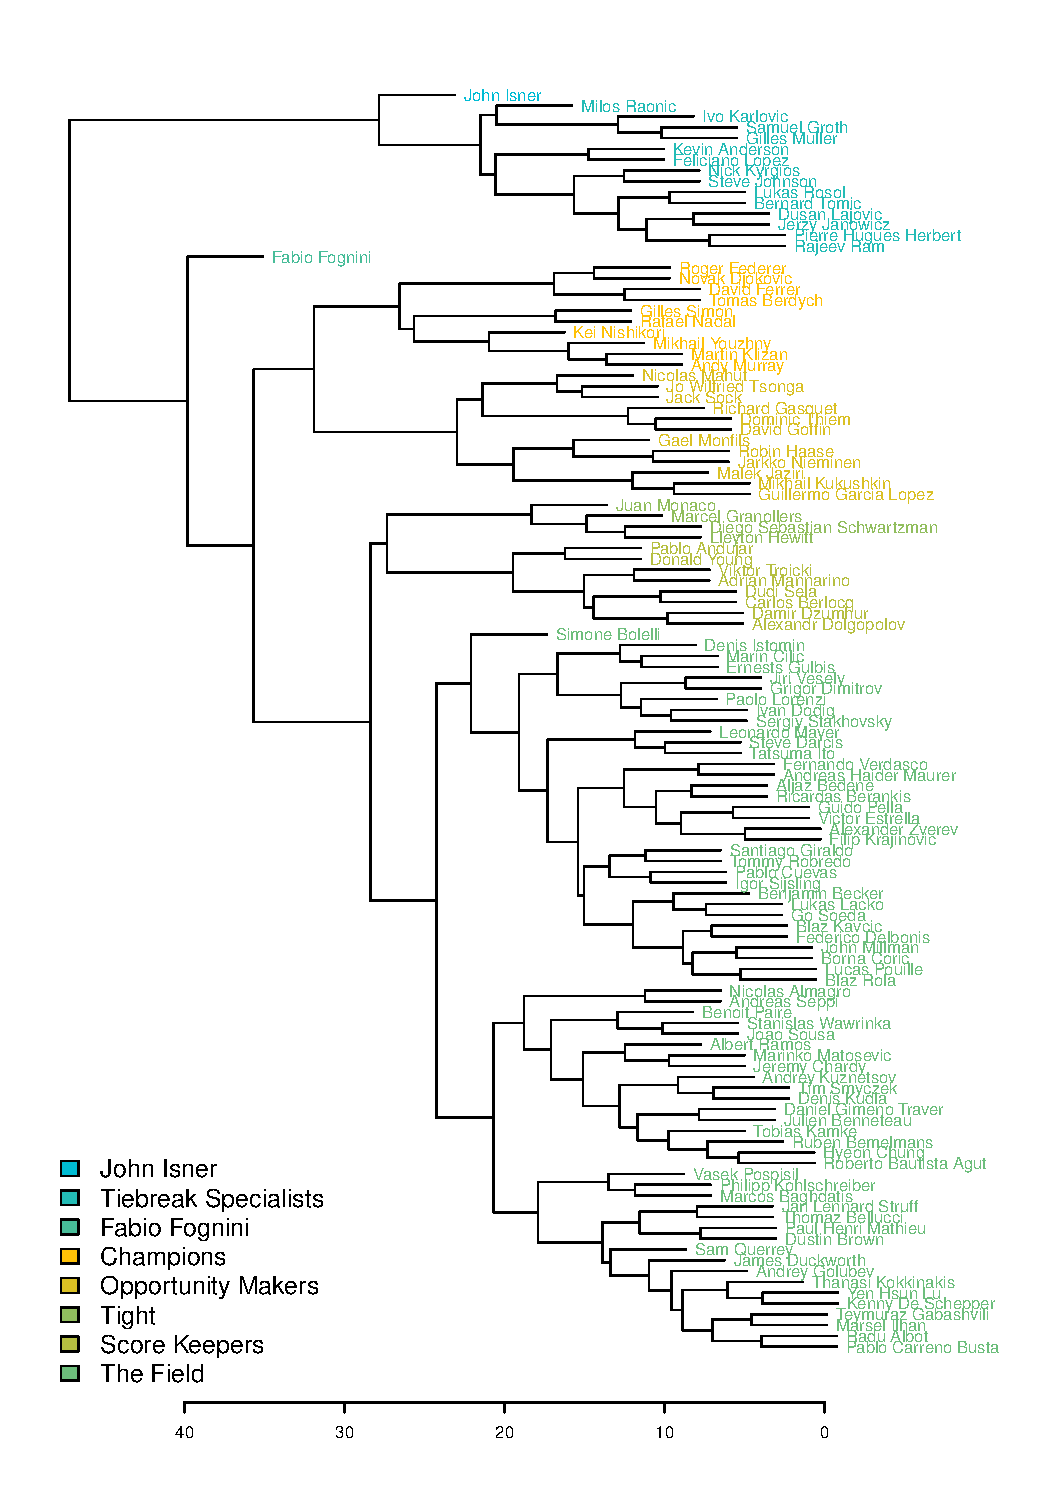
\includegraphics[scale=0.9]{figs/atp_dendro_std_fixed.pdf}
\caption{Dendrogram of distances in ATP mentality profiles for players competing
  in the 2015 Grand Slams. Profiles consisted of 8 dynamic predictors on the
  service game and 8 on the return game. Dissimilarity was measured with a
  manhattan distance and players were clustered using complete linkage.}
\label{fig:atp_dendro}
\end{figure}

\clearpage

\begin{figure}
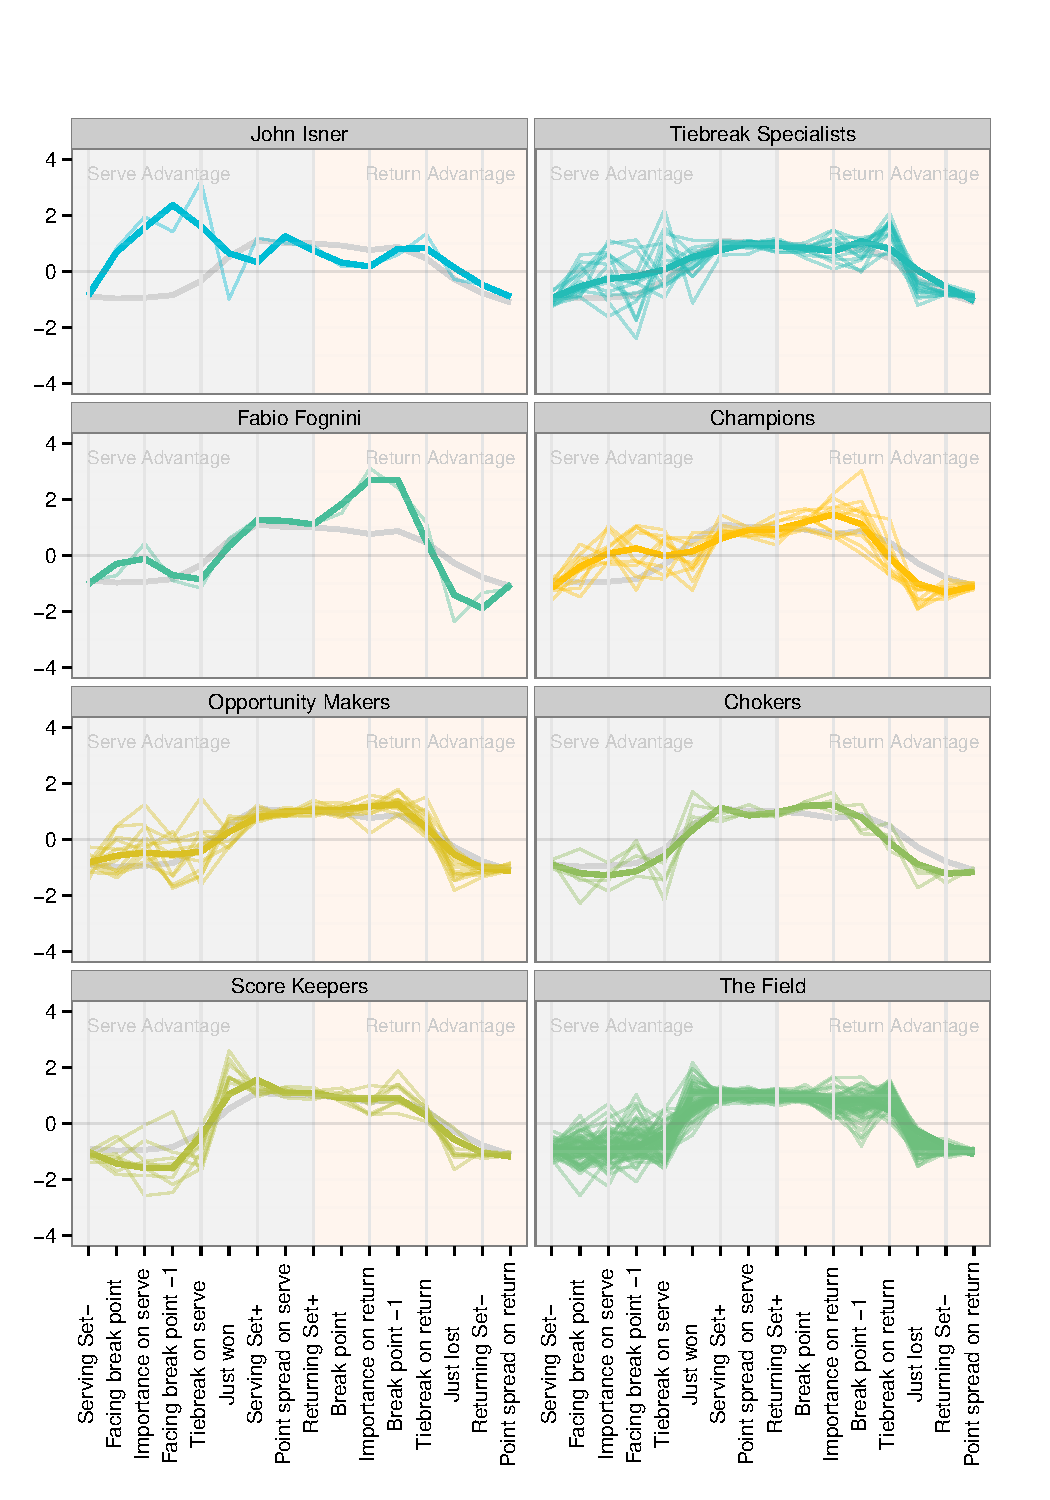
\includegraphics[scale=0.9]{figs/atp_coords_std_fixed.pdf}
\caption{Parallel coordinates plot of mentality types for the ATP players
  represented in the dendrogram of Figure~\ref{fig:atp_dendro}. Effects were
  scaled to have a common standard deviation of one but were not centered so
  that the direction is the direction of the shift in the serve or return
  advantage.}
\label{fig:atp_coord}
\end{figure}

\clearpage

\begin{figure}
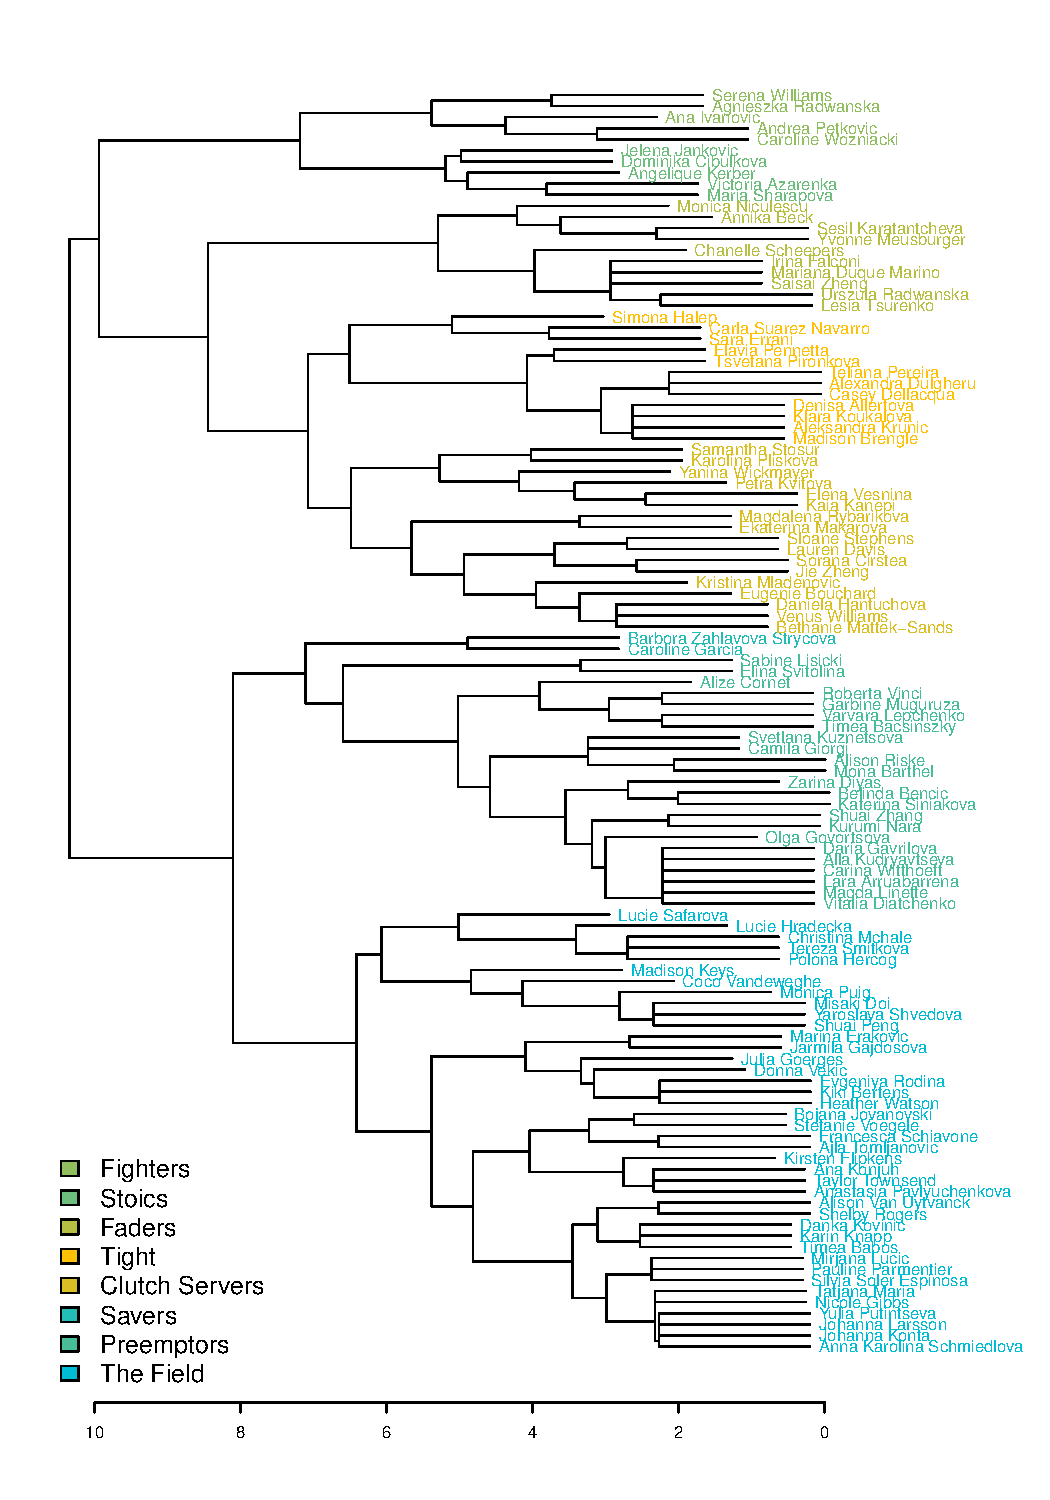
\includegraphics[scale=0.9]{figs/wta_dendro_std_fixed.pdf}
\caption{Dendrogram of distances in WTA mentality profiles for players competing
  in the 2015 Grand Slams. Profiles consisted of 6 dynamic predictors on the
  service game and 6 on the return game. Dissimilarity was measured with a
  manhattan distance and players were clustered using complete linkage.}
\label{fig:wta_dendro}
\end{figure}

\clearpage

\begin{figure}
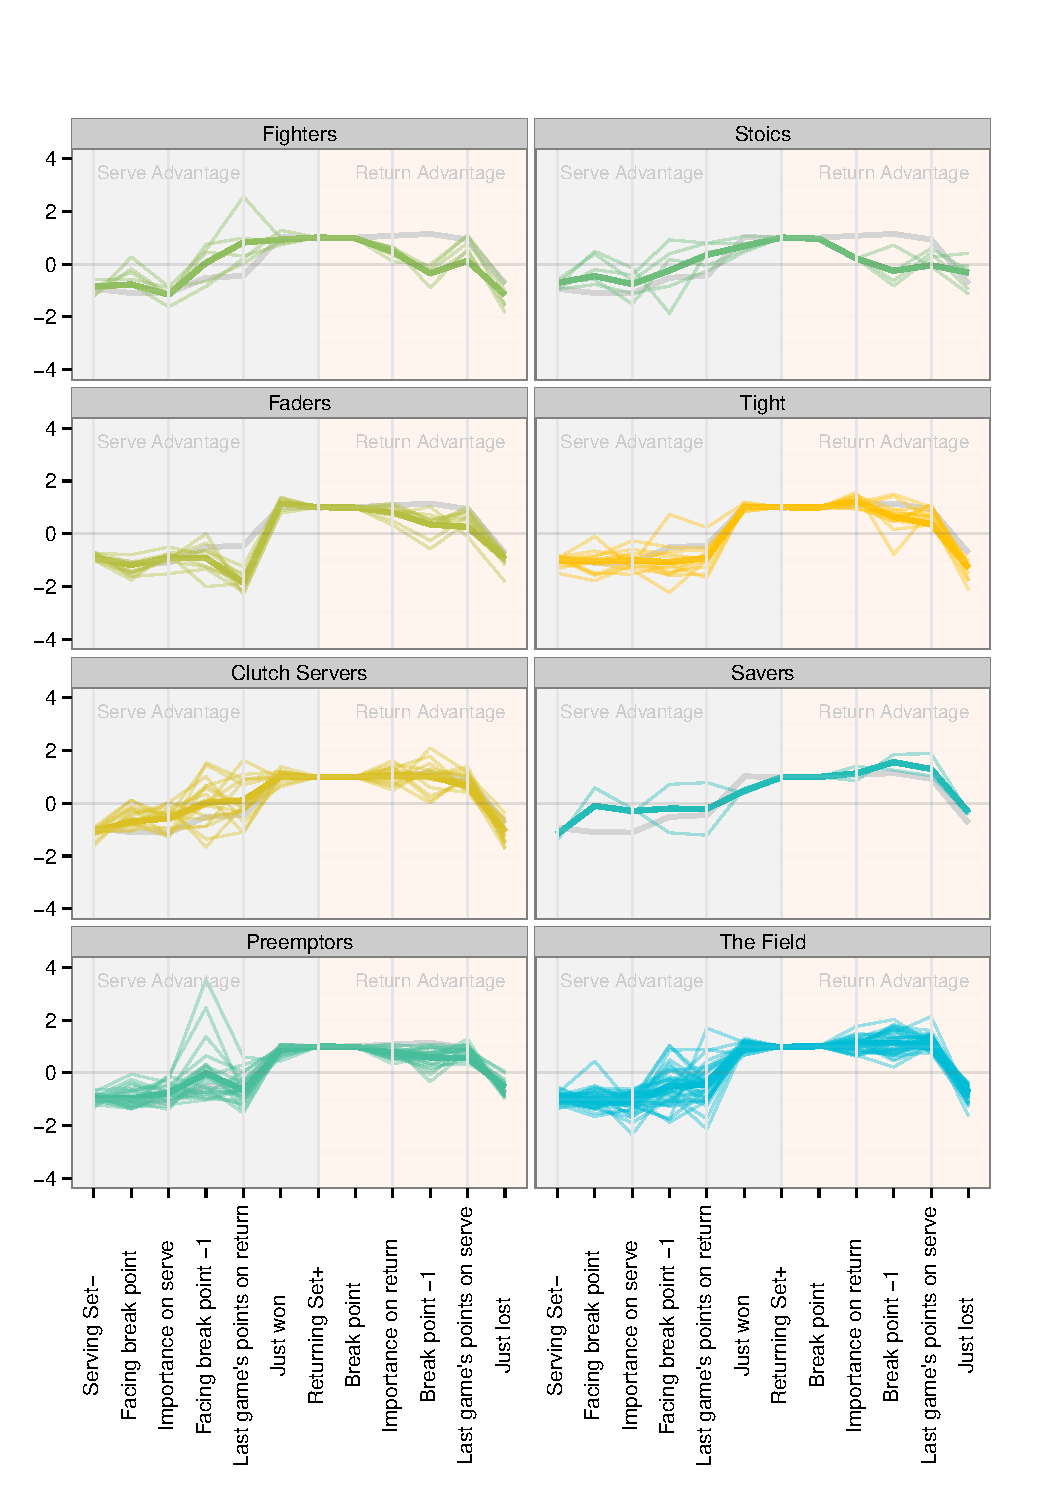
\includegraphics[scale=0.9]{figs/wta_coords_std_fixed.pdf}
\caption{Parallel coordinates plot of mentality types for the WTA players
  represented in the dendrogram of Figure~\ref{fig:wta_dendro}. Effects were
  scaled to have a common standard deviation of one but were not centered so
  that the direction is the direction of the shift in the serve or return
  advantage.}
\label{fig:wta_coord}
\end{figure}

\clearpage

\begin{figure}
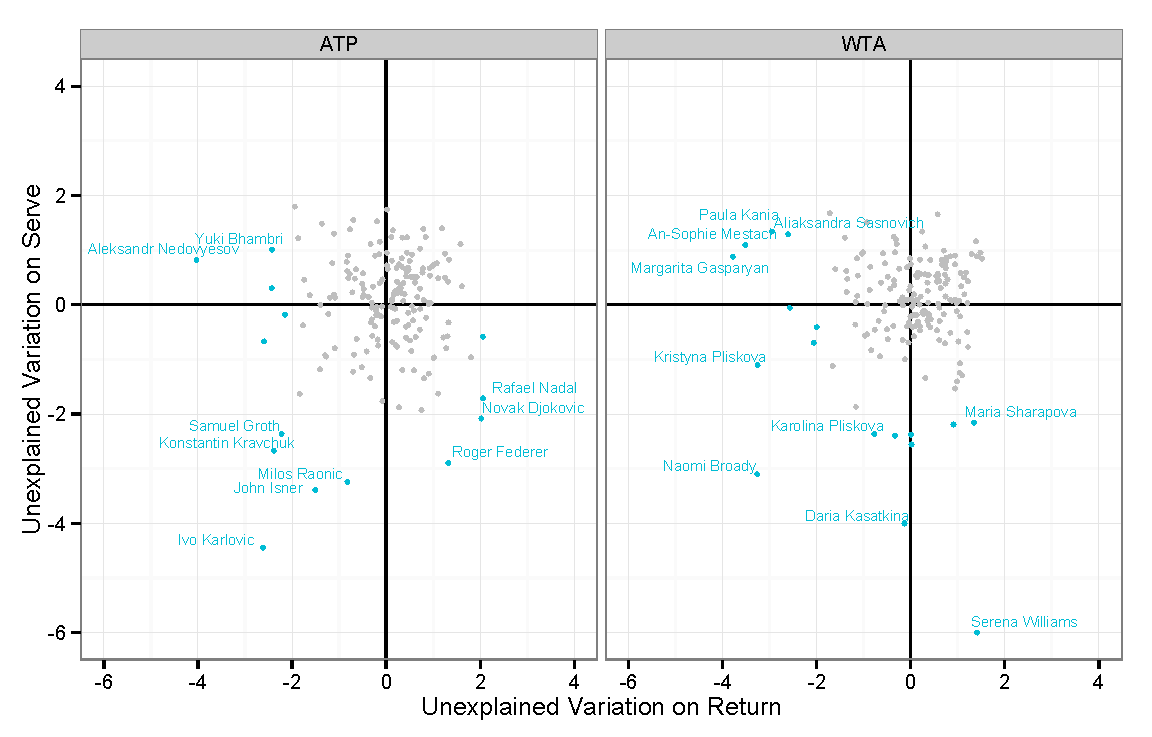
\includegraphics[scale=0.9]{figs/player_volatility.pdf}
\caption{Unexplained variance on serve and return according to the PDM Brier
  scores for each player when applied to the Grand Slam validation data. Brier
  scores are shown as z-scores and outliers with magnitude of 2 or more are
  highlighted in blue. The ten most extreme outliers for each tour are labeled.}
\label{fig:volatility}
\end{figure}

\end{document}
